\documentclass[11pt]{article}

\pagestyle{plain} \textheight 9.0in\headsep -0.50in
\textwidth 6.5in\oddsidemargin 0.0in\evensidemargin 0in
\parindent0pt
\parskip5pt
%this is just a test! Ivo 5-5-2009


%\def\citeusmark{$^{\textstyle \star}$}
%\def\citeus#1#2{\cite{#1}}

%\def\crow#1#2{#2}
%
\usepackage{wrapfig}
\usepackage{multirow}
\usepackage[dvips]{graphicx}
\usepackage{epstopdf}
\usepackage{color}
\usepackage{amsfonts}
\usepackage{amsmath}
\usepackage{url}
\usepackage{amssymb}
\usepackage{subfigure}
\usepackage{comment}
\DeclareGraphicsRule{.tif}{png}{.png}{`convert #1 `dirname #1`/`basename #1 .tif`.png}

\def\cq{{\emph{Culex quinquefasciatus} }}
%


\title{An Agent-Based Model of Host Odor-Mediated Host-Seeking Behavior of Mosquitoes}
\author{
\textbf{Ricardo Cortez}\\
   \small{Mathematics Department}\\
   \small{Tulane University}\\ \and
\textbf{Angela Gallegos}\\
   \small{Mathematics Department}\\
   \small{Occidental College}\\ \and
\textbf{Cavin Ward-Caviness}\\
   \small{Mathematics Department}\\
   \small{Tulane University}\\ \and
\textbf{Ivo M. Foppa}\\
   \small{Department of Epidemiology}\\
   \small{Tulane University}\\
}


\begin{document}

\maketitle

\renewcommand{\labelenumi}{(\alph{enumi})}
\section{Introduction}
%{\bf Mosquito--host ratio.}
%Just a first try--didn't get very far ... 5-30-2009 IF
West Nile virus (WNV), a flavivirus of the Japanese encephalitis virus serocomplex \cite{Petersen2001}, emerged in North America well beyond its traditional Old World range ten years ago and has since become by far the most common cause of arboviral illness in the US and Canada. The virus, which cycles between birds and culicine mosquitoes, has extensively been studied. Yet, the reasons for its epidemiological success remain elusive. Mathematical models of WNV transmission may provide insight into the dynamic peculiarities that set the epidemiology of WNV apart from viruses that are perpetuated similarly. Current models \cite{Wonham2006,Bowman2005} do  not capture spatial heterogeneity of transmission which may be an important aspect of arbovirus perpetuation. In order to gain a deeper understanding of contact process that underlies WNV transmission, i.e. the location of vector mosquitoes, such as {\it Culex quinquefasciatus}, of and subsequent feeding in reservoir hosts (typically birds) we developed an agent-based simulation model of the host seeking behavior of mosquitoes, given two combined odor plumes that are generated by two groups of hosts (``birds'').


%%%%%%%%%%%%%%%%%%%%%%%%%%%%%%%%%%%
\subsection{The Mathematical Model}
%%%%%%%%%%%%%%%%%%%%%%%%%%%%%%%%%%%
The model can be described in terms of three components: (1) the evolution of a concentration
plume used by the mosquitoes to seek out hosts, (2) the behavior of the hosts, and (3) the
behavior of the mosquitoes.  The transmission dynamics is assumed to occur in a two-dimensional
rectangular region whose sides are of length $L_x$ and $L_y$. A population of $N_v$ mosquitoes
(e.g. {\sl Cx. quinquefasciatus}) are initially placed in a subregion that can be selected by
the user. Similarly, there are initial populations of $N_h$ hosts (e.g. birds), placed in
several subregions.


{\bf The odor plume.} The first component of a transmission dynamics model is the mosquito-host
interaction, including the mechanisms that mosquitoes use to find hosts.  Our model is based on
the assertion that hosts release a fixed amount of CO$_2$ (or some other gaseous clues) per host per
unit time.  This concentration plume is then diffused and possibly convected by wind within the
two-dimensional region. The convection velocity of the wind is assumed to be represented by
the known velocity vector ${\vec U}(x,y,t)$.  The concentration $C(x,y,t)$ satisfies the
advection-diffusion equation
\begin{equation}\label{eq:conv-diff}
\frac{\partial C}{\partial t} + {\vec U}\cdot\nabla C = D\nabla^2 C + S(x,y),
\end{equation}
where $t$ is time, and $(x,y)$ are spatial coordinates.  $D$ is the (constant) diffusion coefficient
and can be adjusted to reflect the speed at which the particular substance of interest diffuses in air.
The transport velocity ${\vec U}$ can be used to introduced drifts or relatively large features
produced by the air, but in this case it does not represent small scale turbulence.  The last term
represents the source of CO$_2$ concentration at the host locations. In our model, we will consider
this term to be $S(x,y) = S_0 \sum \delta(x-x_h,y-y_h)$ where $S_0$ is a constant concentration per
unit time and the delta function reflects the fact that the CO$_2$ occurs only at the host locations.
%
Although Eq.~(\ref{eq:conv-diff}) is continuous in space and time, to simulate this spread
computationally, we use a discrete grid of spacing $h$ that covers the two-dimensional
domain $L_x \times L_y$. We use $x_j = jh$ and $y_k = kh$ (with $h N_x = L_x$ and $h N_y = L_y$.
Then $C^n_{j,k}$ approximates $C(x_j,y_k,t_n)$ and its derivatives are approximated
using center-differences:
\[
\frac{\partial C}{\partial x}(x_j,y_k,t_n) \approx \frac{ C^n_{j+1,k} - C^n_{j-1,k} }{2h},
\hskip20pt
\frac{\partial^2 C}{\partial y^2}(x_j,y_k,t_n) \approx \frac{ C^n_{j,k+1} - 2C^n_{j,k} + C^n_{j,k-1} }{h^2},
\hskip20pt etc.
\]

{\bf The host behavior.} The principal opportunities for host-mosquito interaction are during roosting periods in which hosts are relatively stationary. This assumption is based on the crepuscular and nocturnal feeding habits of \cq. Our model allows the hosts a small random motion about their roosting location. At fixed time
intervals, the steps of this random walk are selected from a Gaussian distribution with zero mean and adjustable variance. The direction of each step is given by an random angle $\theta$ taken from a uniform distribution
between $0$ and $2\pi$.  Currently, the random steps in all directions are equally likely; however,
enhancements to this component such as biasing the random walk to account for preferred motion of the hosts can easily be included.

{\bf The mosquito behavior.} A random walk with zero mean and its own variance is also applied to the mosquitoes to describe small-scale behavior not accounted for in other parts of the model.  In addition, the mosquito behavior includes a host-seeking component that allows them to find hosts. Neither the host nor the mosquito
locations are restricted to the CO$_2$ grid. We assume that the mosquitoes can sense {\em the direction
of the concentration gradient} of the CO$_2$ with an accuracy depending on the magnitude of the gradient.
Larger gradients are sensed with better accuracy than lower ones.
This sensing mechanism is accounted for by introducing a second random walk of the mosquitoes
in a direction approximately equal to that of the concentration gradient.
%
For example, we assume that the concentration gradient at the
mosquito location $(x,y)$ is $\nabla C(x,y)$ in the direction of an angle $\theta$
(see Figure~\ref{MosquitoGradient}).
The mosquito at that location takes a step of fixed size in a direction given
by a random angle in the interval $[\theta-\alpha, \theta+\alpha]$.  The size of this window,
represented by $\alpha$, is smaller when the concentration gradient magnitude $|\nabla C|$ is large.
Specifically, we use
\[
\alpha = \alpha_{min} + \frac{ \alpha_{max}-\alpha_{min}}{1 + \beta|\vec{U}|}
\]
so that the extreme cases of $|\nabla C|=\infty$ and $|\nabla C|=0$ give
$\alpha_{min}$ and $\alpha_{max}$, respectively. In this equation, $\beta$ is a constant with
the appropriate units to make the expression dimensionless.

\begin{figure}[hbtp]
\centering
 \includegraphics[width=.2\textwidth]{figures/GradientWalkSchematic.ps}
\caption{Schematic of the mosquito host-seeking model based on the concentration gradient direction.}
\label{MosquitoGradient}
\end{figure}


{\bf The biting rate.} Once a mosquito comes in contact with a host, there is a possibility of
a blood meal and transmission of the infection.  In our model, the
mosquitoes and hosts are represented by points moving in space; thus,  they do not actually come into
contact. However, we define a ``biting radius" around each mosquito.  If a mosquito is within the biting radius of the host, it has a possibility of biting it.  The biting radius is a purely computational parameter so
there is a need to determine its appropriate range of values through
numerical tests.  Once a host is within the biting radius of a mosquito, we
assign both a probability of a blood meal and a probability of transmission (in the case that
the encounter involves one infectious and one susceptible agent).
The mosquito-to-host transmission and the host-to-mosquito transmissions
occur with different probabilities.  Hosts recover from infection at a given rate and
no host mortality was assumed to occur.

In summary, the model consists of the following equations for the hosts locations $(x_h,y_h)$,
the mosquito locations $(x_m,y_m)$ and the CO$_2$ concentration $C$:
\begin{eqnarray*}
\mbox{Hosts:}&&
\frac{dx_h}{dt} = \ell_h \cos(\phi_u),
\hskip20pt
\frac{dy_h}{dt} = \ell_h \sin(\phi_u) \\
\mbox{Mosquitoes:}&&
\frac{dx_m}{dt} = \ell_m \cos(\psi_u) + d_m \cos(\alpha_u),
\hskip20pt
\frac{dy_m}{dt} = \ell_m \sin(\psi_u) + d_m \sin(\alpha_u) \\
\mbox{Concentration:}&&
\frac{\partial C}{\partial t} + U_1\frac{\partial C}{\partial x}
+ U_2\frac{\partial C}{\partial y} =
D\left( \frac{\partial^2 C}{\partial x^2} + \frac{\partial^2 C}{\partial y^2} \right)
+ S_0 \sum\delta(x-x_h,y-y_h)
\end{eqnarray*}
where $\ell_h$, $\ell_m$ and $d_m$ are fixed distances, all angles with a subscript
$u$ are random variables with uniform distribution; $\phi_u$ and $\psi_u$ take
values in $[0,2\pi)$ and $\alpha_u$ takes values in $(\theta-\alpha,\theta+\alpha)$
as described earlier.  The wind transport is represented by $\vec{U}$ and is assumed
to be known, $D$ is the diffusivity of the concentration $C$ in air, and
$S$ is the CO$_2$ source (constant per host per unit of time) at the host locations.

The equations are coupled together since the host locations affect the concentration
gradient, which in turn, affects the motion of mosquitoes.  Once a mosquito is
within the biting radius $R_b$ of a host, there is a probability $P_b$ of biting.
After biting, there is a probability $P_t$ of transmission to the host.  Both of
these probabilities are assumed to be constant. Once a mosquito has bitten a host,
it no longer participates in the dynamics (one blood meal per mosquito).


%%%%%%%%%%%%%%%%%%%%%%%%%%%%%%%%%%%%
\subsubsection{Dimensionless representation of the model}
%%%%%%%%%%%%%%%%%%%%%%%%%%%%%%%%%%%%
In order to reduce the number of parameters in the model, we define dimensionless
versions of all variables by choosing appropriate scalings. We choose the velocity
scale to be $d_m$, the mosquito host-seeking speed, and the length scale to be
the size of the domain $L$.  Together they define a time scale given by
$T = L/d_m$.  We also choose a concentration scale based on the rate of CO$_2$
production per host per time, $S_0T$.  In this way, the dimensionless
concentration is related to the dimensional concentration by $\hat{C} = C/(S_0T)$.
Similarly, all variables with units of length are divided by $L$.
The equations in dimensionless form are
\begin{eqnarray*}
\mbox{Hosts:}&&
\frac{dx_h}{dt} = \xi \cos(\phi_u),
\hskip20pt
\frac{dy_h}{dt} = \xi \sin(\phi_u) \\
\mbox{Mosquitoes:}&&
\frac{dx_m}{dt} = \gamma \cos(\psi_u) + \cos(\alpha_u),
\hskip20pt
\frac{dy_m}{dt} = \gamma \sin(\psi_u) + \sin(\alpha_u) \\
\mbox{Concentration:}&&
\frac{\partial C}{\partial t} + V_1\frac{\partial C}{\partial x}
+ V_2\frac{\partial C}{\partial y} = \mu
\left( \frac{\partial^2 C}{\partial x^2} + \frac{\partial^2 C}{\partial y^2} \right)
+ \sum\delta(x-x_h,y-y_h) \\
&& \alpha = \alpha_{min} + \frac{ \alpha_{max}-\alpha_{min}}{1 + \rho|\nabla C|}
\end{eqnarray*}
where the dimensionless groups are,
\[
\xi = \frac{\ell_h}{d_m},
\hskip10pt
\gamma = \frac{\ell_m}{d_m},
\hskip10pt
\mu = \frac{D}{d_m L},
\hskip10pt
\rho = \frac{\beta S_0}{d_m},
\hskip10pt
V_i = \frac{U_i}{d_m}
\]

%%%%%%%%%%%%%%%%%%%%%%%%%%%%%%%%%%%%
\subsubsection{Example: Parameter study}
%%%%%%%%%%%%%%%%%%%%%%%%%%%%%%%%%%%%
We begin with an example that will help gain insight into the effect of the
parameters in host-seeking behavior.  In this case, the hosts will be stationary,
so we set $\xi = 0$, and we assume there is no advection ($V_1 = V_2 = 0$).
We fix the value of $\mu$ and study the effect of $\gamma$ and $\rho$.  The setup
consists of two groups
of hosts containing 90\% and 10\% of the hosts, respectively, placed initially
at the same distance from the release location of the mosquitoes.  As we vary the
parameters, we record the number of mosquitoes that bite hosts in each of the groups.





\begin{figure}[hbtp]
     \centering
     \subfigure[]{
          \label{fig:ex1a1}
          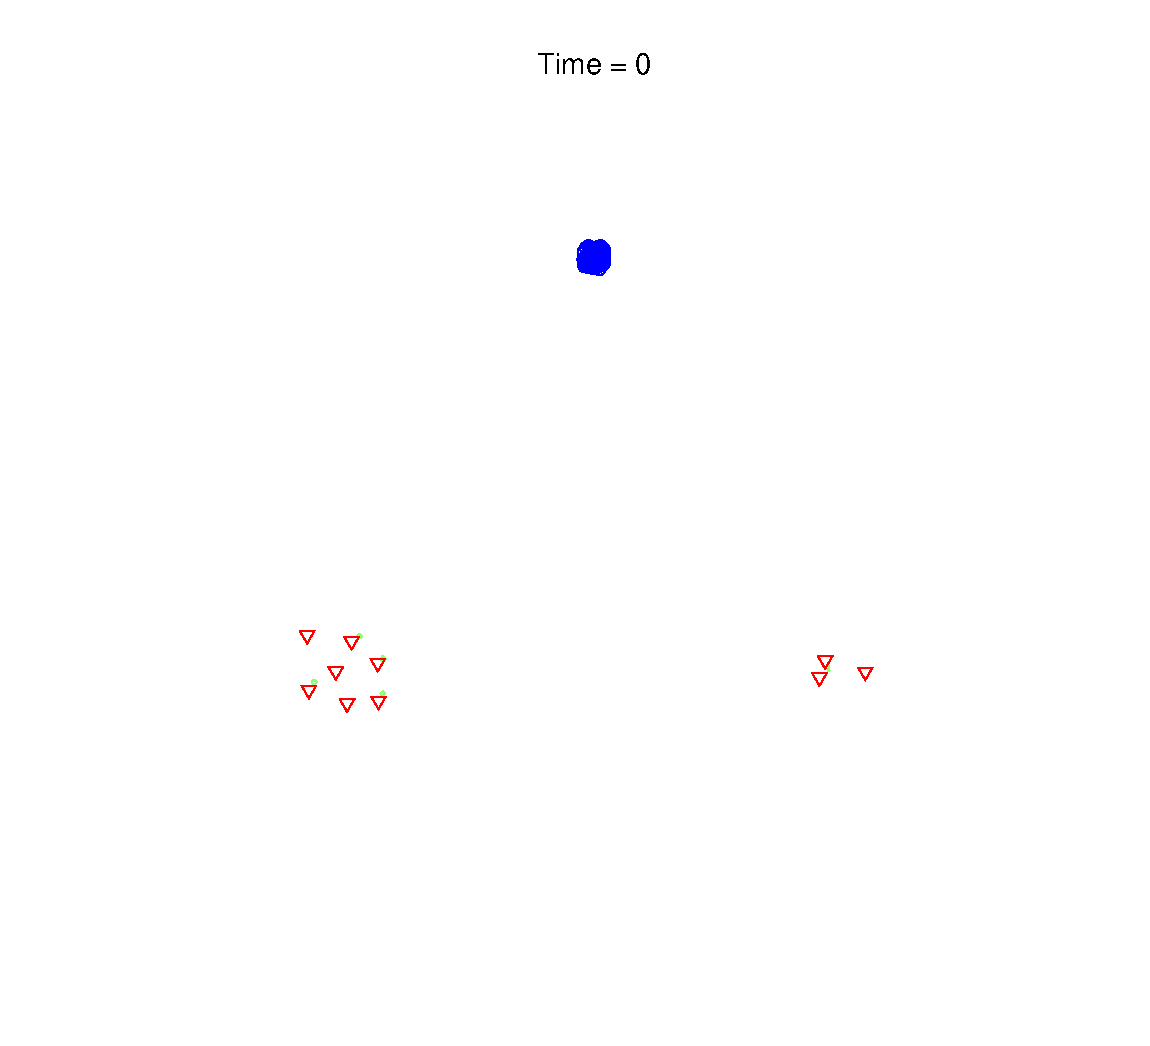
\includegraphics[width=.32\textwidth]{figures/ExA1.eps}}
     %\hspace{.2in}
     \subfigure[]{
          \label{fig:ex1a2}
          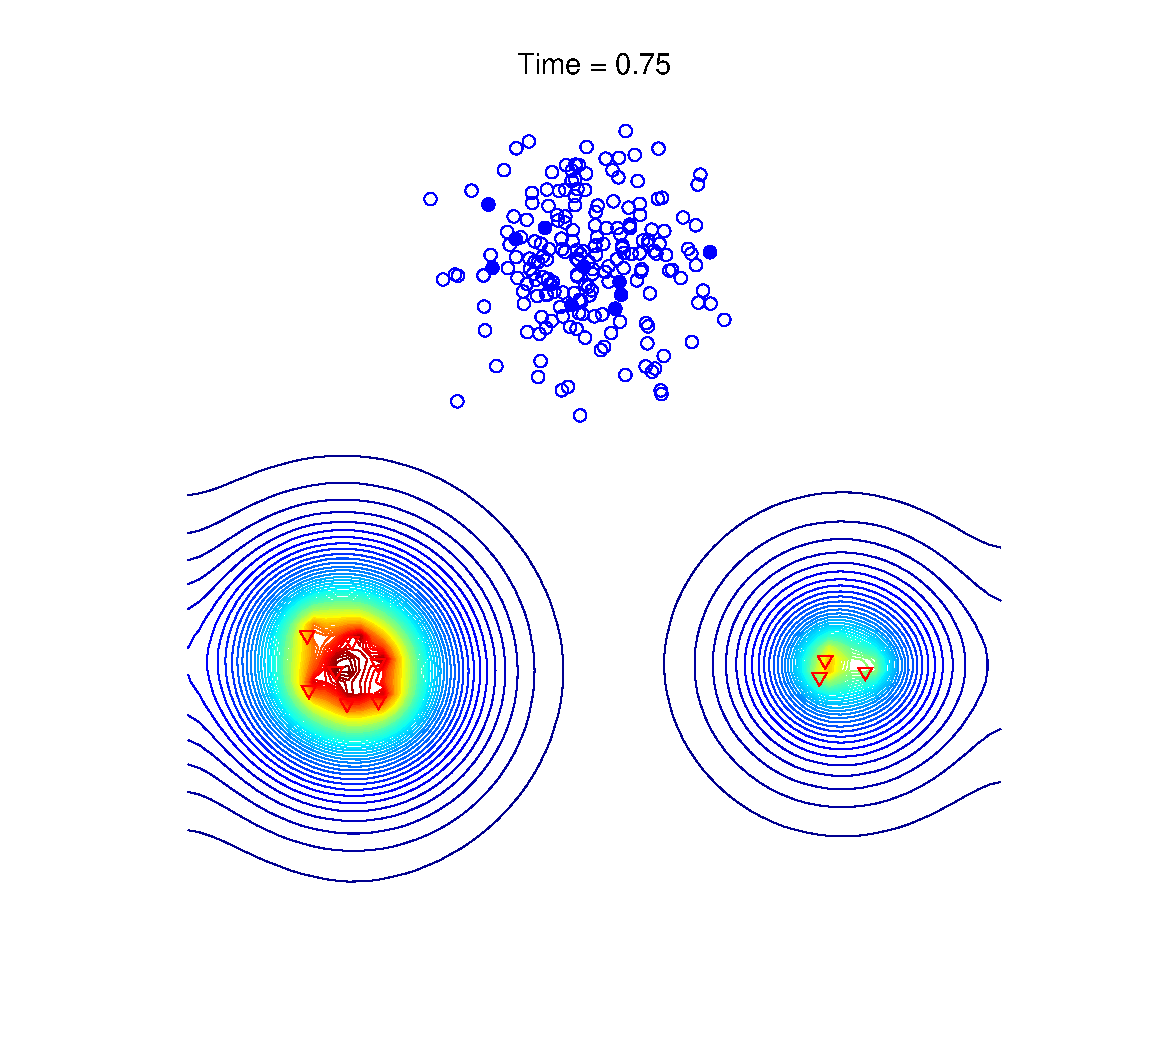
\includegraphics[width=.32\textwidth]{figures/ExA4.eps}}
     %\hspace{.2in}
     \subfigure[]{
           \label{fig:ex1a3}
           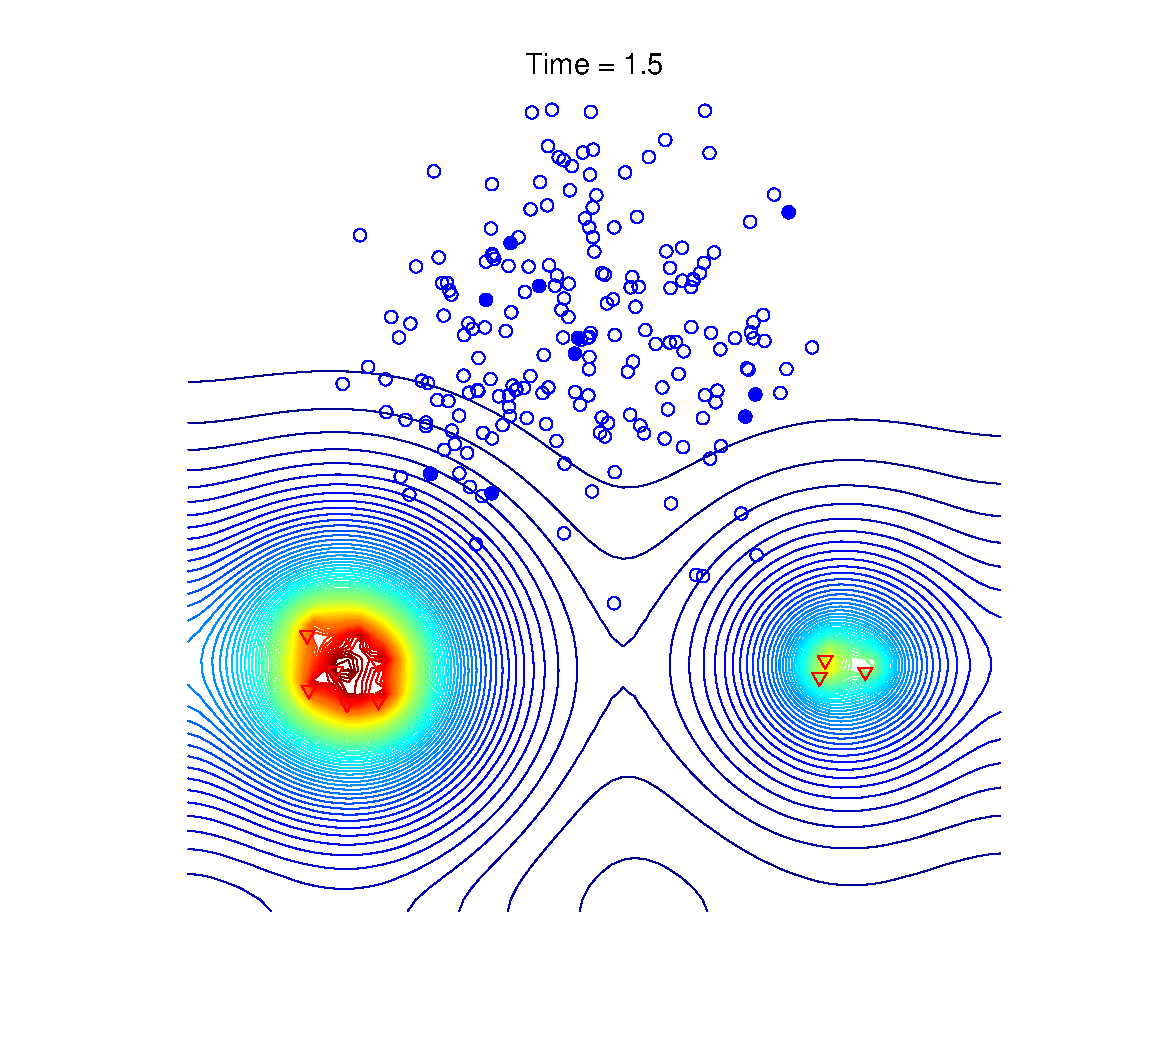
\includegraphics[width=.32\textwidth]{figures/ExA7.eps}}\\
     \subfigure[]{
           \label{fig:ex1a4}
          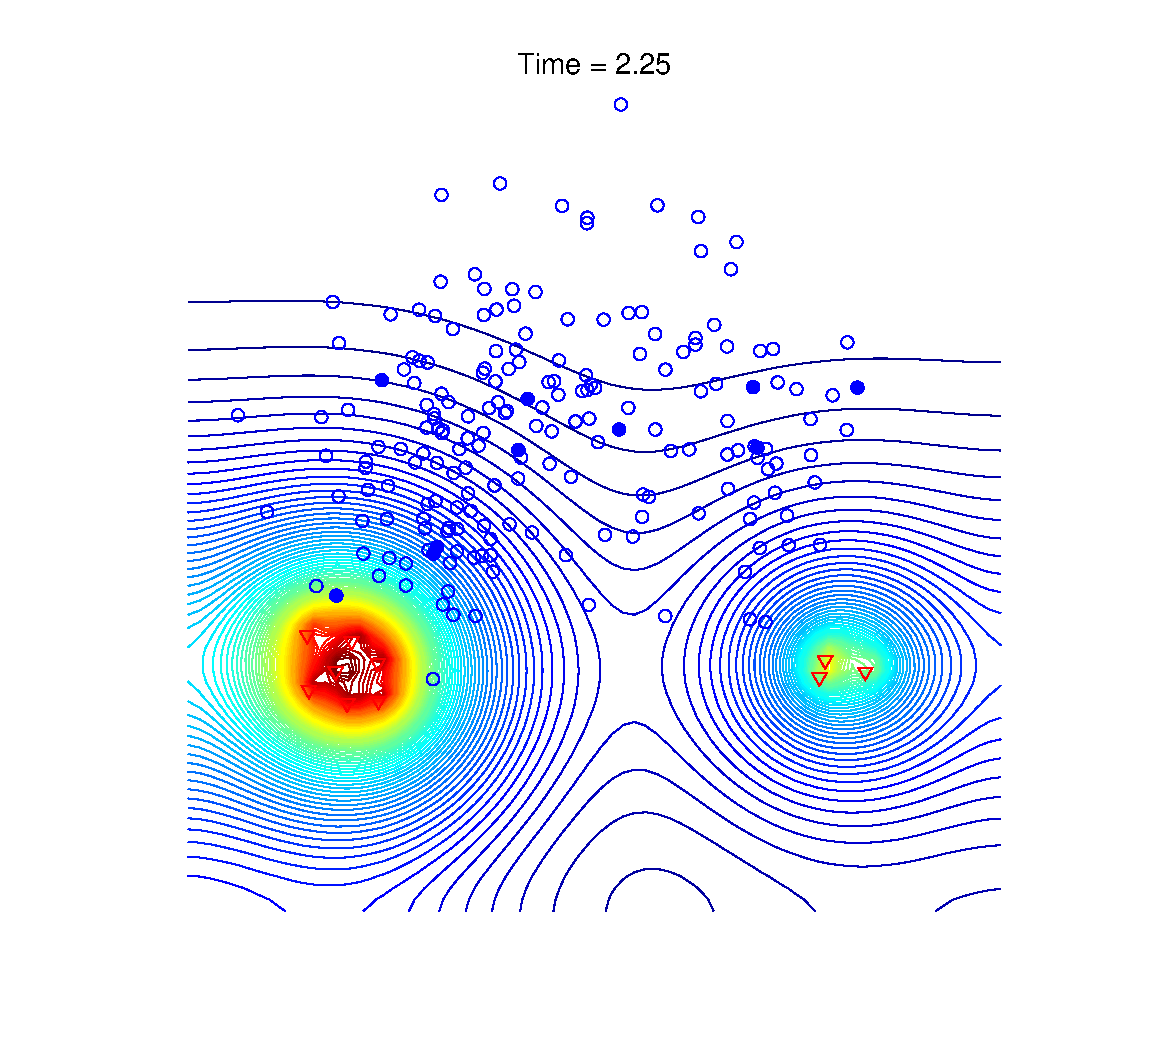
\includegraphics[width=.32\textwidth]{figures/ExA10.eps}}
     %\hspace{.2in}
     \subfigure[]{
           \label{fig:ex1a5}
           \includegraphics[width=.32\textwidth]{figures/ExA13.eps}}
     %\hspace{.2in}
     \subfigure[]{
           \label{fig:ex1a6}
          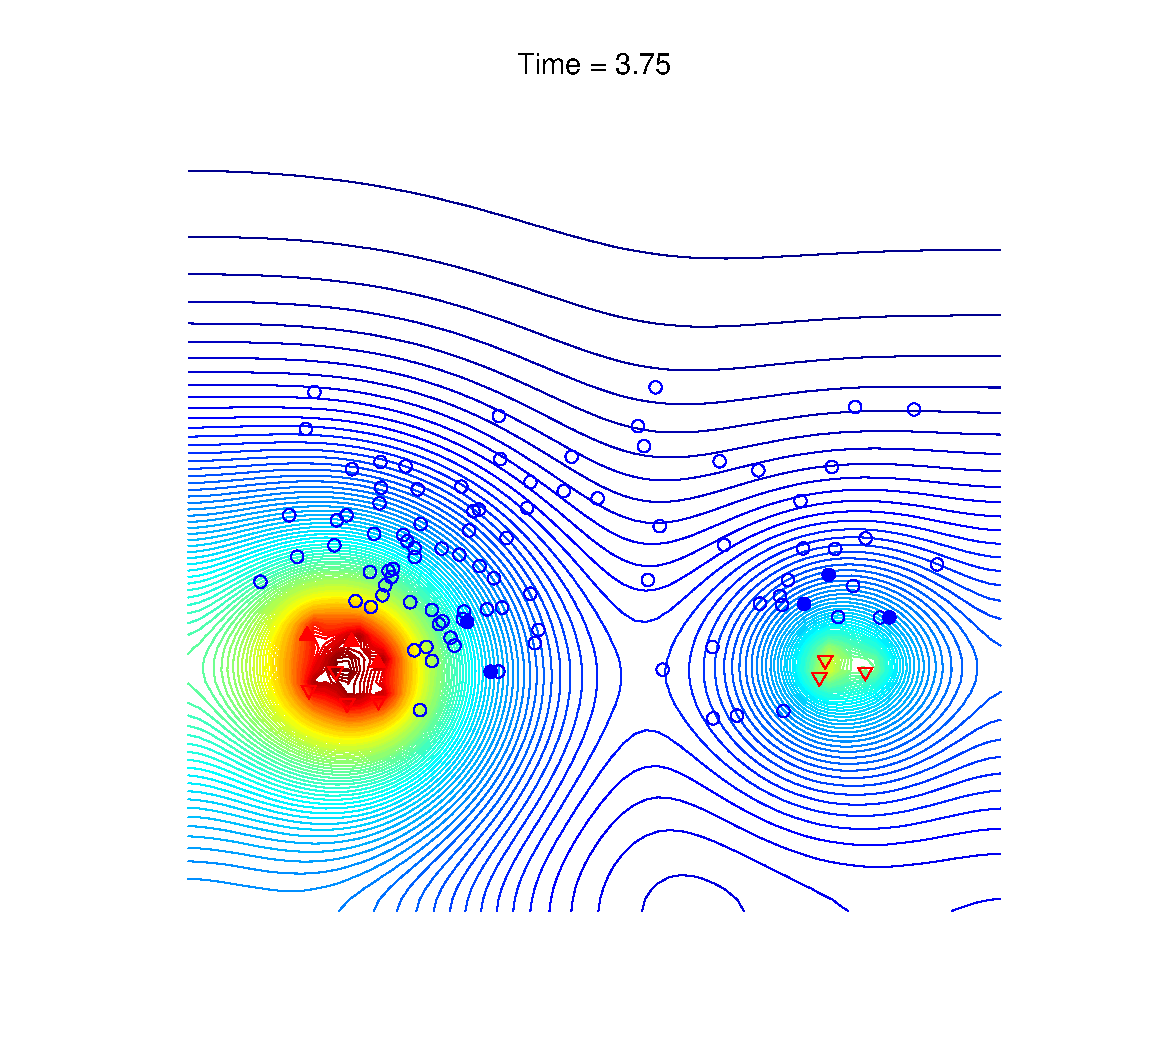
\includegraphics[width=.32\textwidth]{figures/ExA16.eps}}
     \caption{Mosquito and host spatial distribution at various times. The initial host population
was given by two equal groups at equal distances from the mosquito release location.  Vectors seek hosts by moving
in the direction of a concentration gradient plus the random walk. The number of
vectors infected by the larger group is larger but not proportional to the group size.}
     \label{fig:ex1a}
\end{figure}


\begin{figure}[hbtp]
\centering
\includegraphics[width=0.6\textwidth]{figures/Gamma_vary.eps}
\caption{Percentage of mosquitoes that find hosts in the larger group as a function of $\gamma$.
Since $\gamma$ is the ratio of the random walk speed of mosquitoes to the speed of mosquitoes
due to the gradient sensing, the smaller values of $\gamma$ correspond to less dispersion of
mosquitoes during the process. This leads to a larger percentage of them reaching the larger
group of hosts.}
\end{figure}


\begin{comment}
\begin{figure}[hbtp]
\centering
\includegraphics[width=0.75\textwidth]{figures/AveExposedHosts50_50.eps}
\caption{Average percentage of hosts that are exposed to infection.}
\end{figure}


\begin{figure}[hbtp]
\centering
\includegraphics[width=0.8\textwidth]{figures/MosquitoDistribution50_50.eps}
\caption{Average percentage of hosts that are exposed to infection for the 50:50 case.
Notice that approximately half of the mosquitoes are near each group of hosts.}
\end{figure}




\begin{figure}[hbtp]
     \centering
     \subfigure[]{
          \label{fig:ex1b1}
          \includegraphics[width=.4\textwidth]{figures/Ex1Bt1.eps}}
     \hspace{.3in}
     \subfigure[]{
          \label{fig:ex1b2}
          \includegraphics[width=.4\textwidth]{figures/Ex1Bt2.eps}}\\
     \vspace{.3in}
%     \hspace{.1in}
     \subfigure[]{
           \label{fig:ex1b3}
           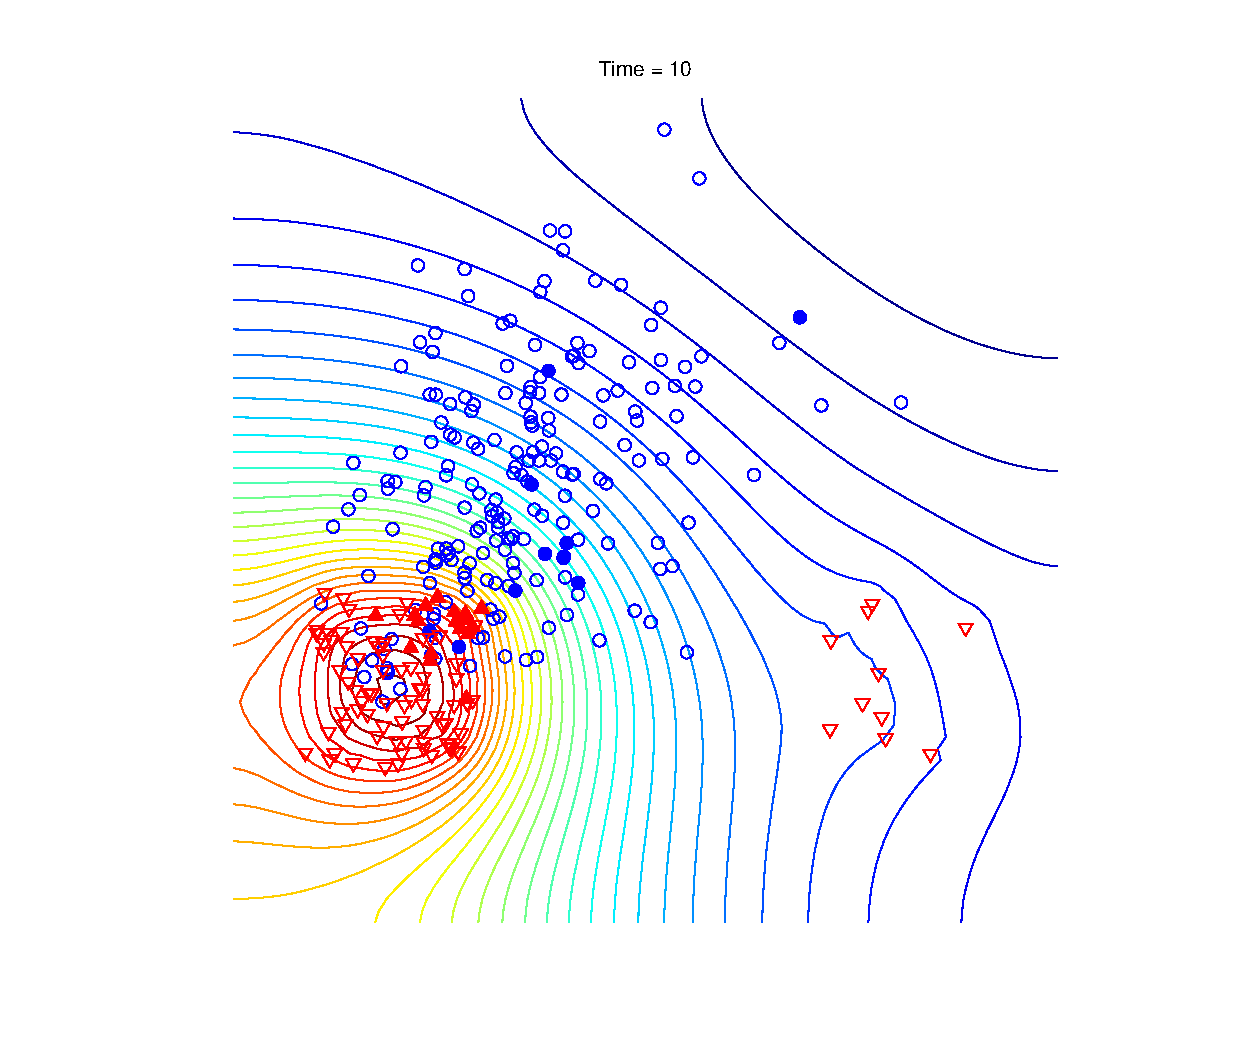
\includegraphics[width=.4\textwidth]{figures/Ex1Bt3.eps}}
     \subfigure[]{
           \label{fig:ex1b4}
          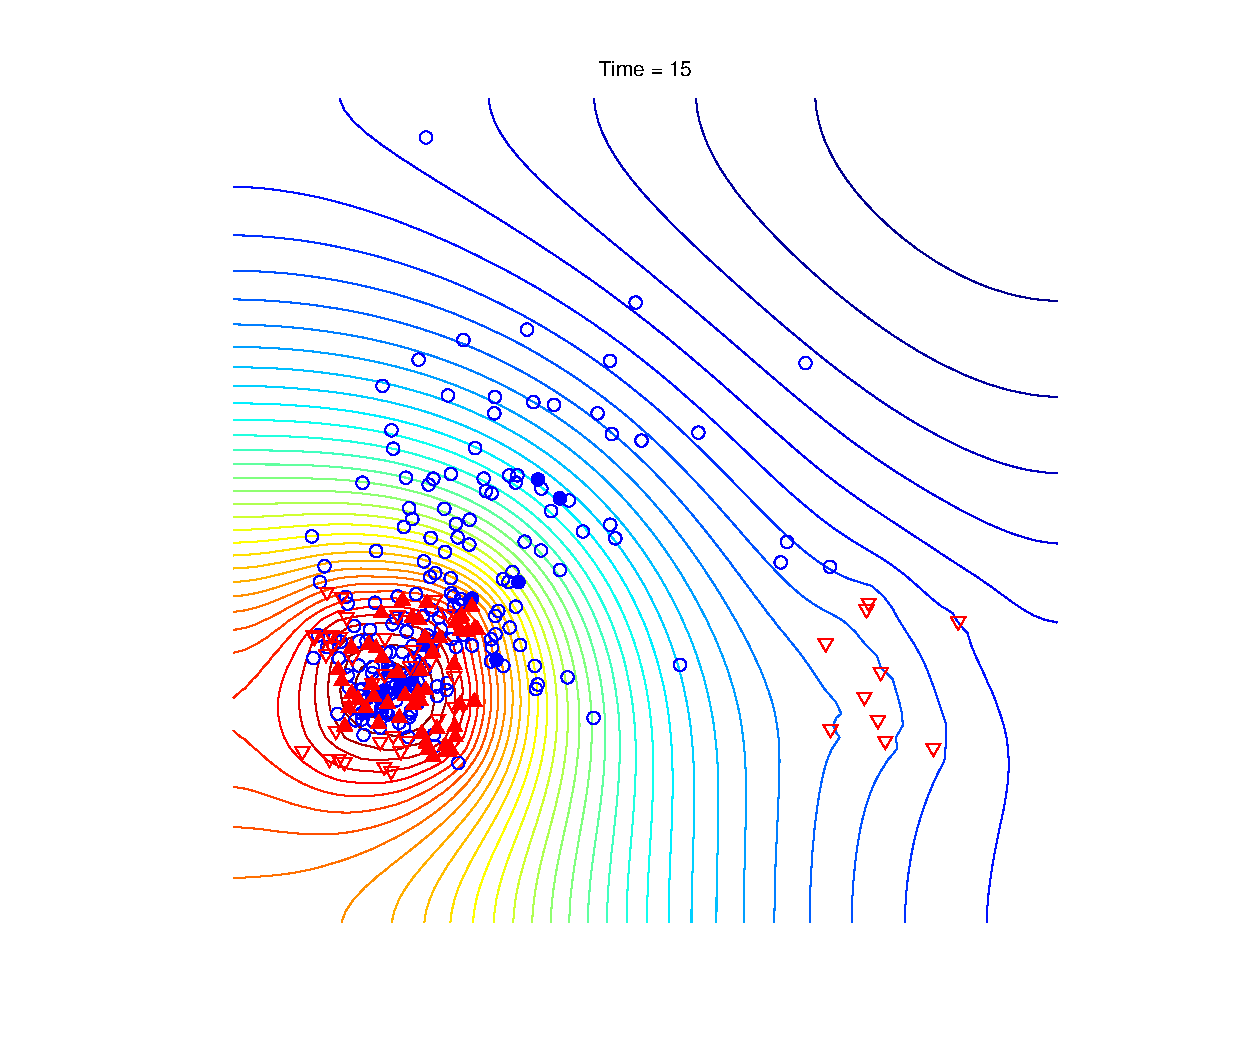
\includegraphics[width=.4\textwidth]{figures/Ex1Bt4.eps}}
     \caption{Mosquito and host spatial distribution at various times. The initial host population
was given by two groups, 90\% on the left and 10\% on the right, at equal distances from the mosquito
release location.}
     \label{fig:ex1b}
\end{figure}

\begin{figure}[hbtp]
\centering
\includegraphics[width=0.75\textwidth]{figures/AveExposedHosts.eps}
\caption{Average percentage of hosts that are exposed to infection for the 90:10 case.}
\end{figure}

\end{comment}


\bibliographystyle{nature}	
\newpage\bibliography{biblio}
\end{document}
